\begin{figure}[t]
\hspace{0.55\textwidth}\begin{minipage}{0.15\textwidth}
\centering \textbf{\colorbox{white}{\scalebox{.7}{Ground-truth}}}
\end{minipage}\begin{minipage}{0.15\textwidth}
\centering \textbf{\colorbox{white}{\scalebox{.7}{Standard}}}
\end{minipage}\begin{minipage}{0.15\textwidth}
\centering \textbf{\colorbox{white}{\scalebox{.7}{AR (ours)}}}
\end{minipage}

\vspace{-0.9 cm}
\subfloat[Proposed Adversarially Robust Model]{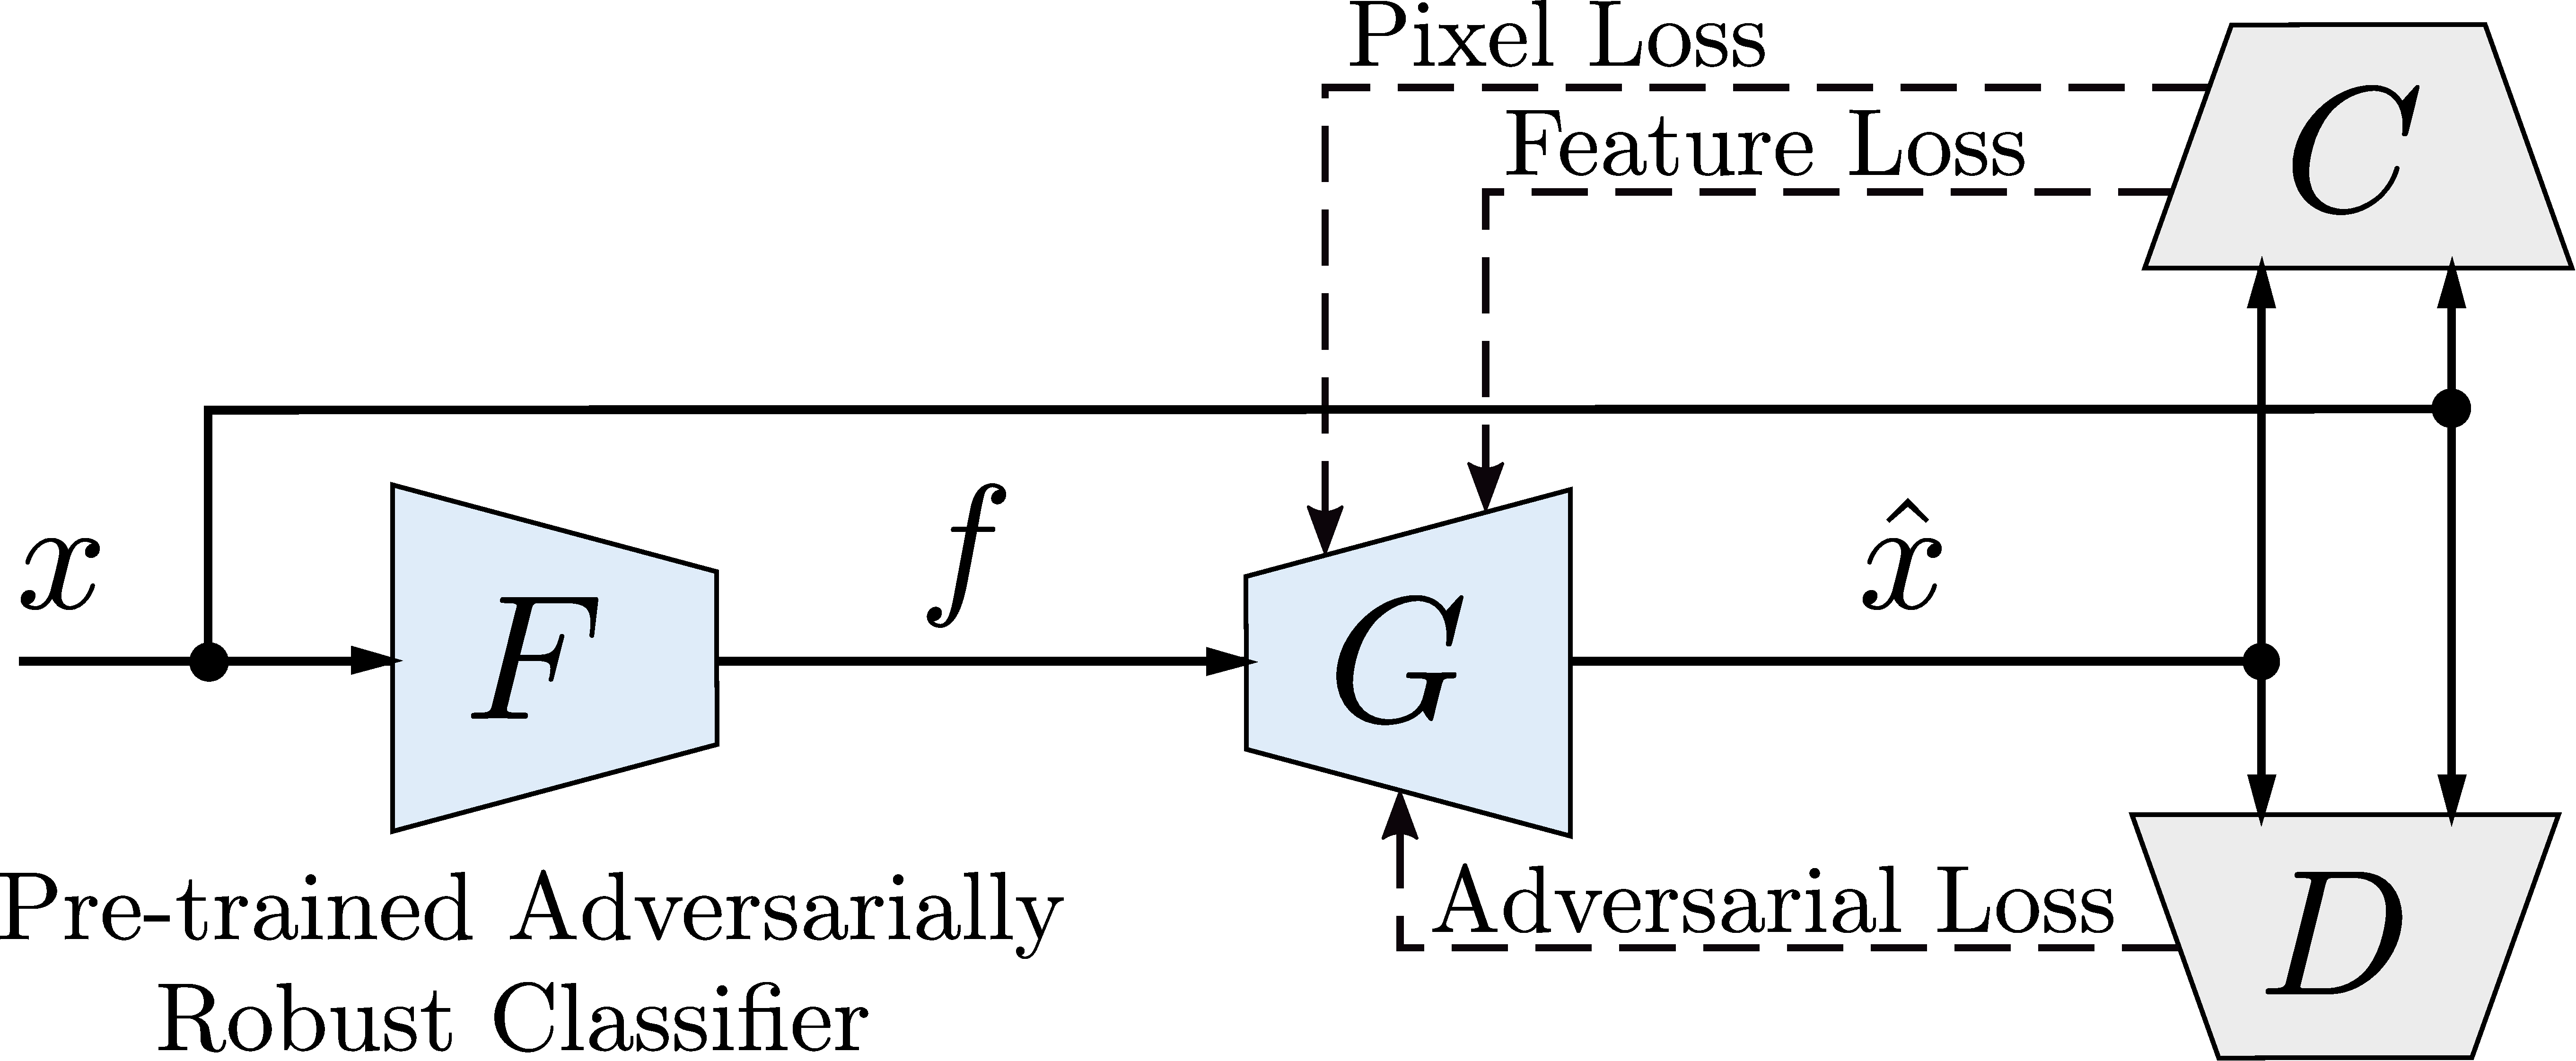
\includegraphics[width=0.45\textwidth]{figs/proposed/encdec.pdf}\hspace{0.1\textwidth}}
\subfloat[Feature Inversion ($224 \times 224$ px.)]{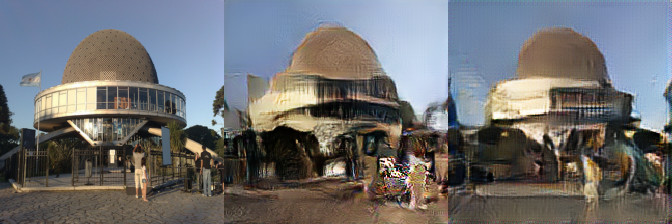
\includegraphics[width=0.45\textwidth]{figs/lowres/tile_inversion.jpg}}


\caption{\label{fig:proposed_model}By training it to invert adversarially robust features, our proposed autoencoder obtains better reconstructions than models trained on standard features.}
\vspace{-0.5cm}
\end{figure}
